\section{Implementing in Python}
In this section, first, the lexer and parser in 
python as a target language will be generated. Then
we Implement a simple and limited Listener that support
some important part of the language. In the next
section we'll elaborate on this and create a browser
base application for that. 
\subsection{Generate lexer and parser in Python}
To make the process straightforward, a 
Gradle-build file is created to do the 
commands. This is the Gradle file script:
\lstinputlisting[style=ANTLR,
caption={Gradle script},
    label={list:gradle}]{../build.gradle}

Two tasks are defined, \textit{generateLexer}, and 
\textit{generateParser} that take proper inputs and 
generate files in a proper path that is 
specified. \textbf{ANTLR_SRC} and 
\textbf{GEN_SRC} are specified in the 
\textit{gradle.properties} file.

\subsection{Setting up a Simple DOT Intepreter}
In the previous section, files 
\textit{DOTLexer.py}, \textit{DOTParser.py} 
and \textit{DOTParserListener.py} were 
generated. So now we'll override 
\textit{DOTParserListener.py} with our own 
Listener in another file is called \textit{GraphDOTListener.py}. Before that, we go through the 
steps of how to use our listener in Python. 
And for that, we need to first install the 
\textbf{antlr4-python3-runtime}. The proper way 
to do that is by using \textit{pip}.

\pythonexternal[ caption=a simple code of 
using our listener with 
passing networkx graph to it, label=list:main1]
{codes/main1.py}

Without further ado, let's look at our code 
that is shown in the Listings \ref{list:main1}. 
From line 1 to line 7, needed modules are 
imported. sys module to read terminal 
arguments for specifying input files. 
antlr4 is our ANTLR runtime and has functions 
for reading inputs from files and walking 
through our Listener function. Our generated 
lexer and parser and then our Listener that 
we'll implement in the next section. 
 

The most important things happen in lines 11 
through 19. In the line 11, characters are 
read from the file. Then these characters plug 
into the lexer to take tokens, and then using 
antlr4, we get the stream of the tokens and pass 
it to the parser to create the parse tree. Then 
the graph is passed to the Listener, and with 
the antlr4 helper functions, we walk through 
the tree to manipulate the graph object.

\subsubsection{Setting up the Listener}

In our first iteration of setting up the 
Listener. We redefine our Language Rules in 
more easier and straightforward terms.
\begin{enumerate}
\item
Our graph is directed or undirected and this is 
defined in the graph rules so we override our
enterGraph:
\begin{python}
def __init__(self):
       self.g = None

def enterGraph(self, ctx:DOTParser.GraphContext):
    if ctx.GRAPH() is not None:
        self.g  = nx.Graph() 
    elif ctx.DIGRAPH() is not None:
        self.g = nx.DiGraph()
    # label property specify the name of the graph
    self.g.graph['label'] = ctx.name().getText()
\end{python}
\item
We can define edges with -- and -> between nodes.
They are not different. if the graph is defined as
directed, they are one-way edge from the first node to 
the second, otherwise they are simple edge.
\begin{python}
def exitEdge_stmt(self, ctx:DOTParser.Edge_stmtContext):
    if ctx.node_name() is not None:
        first_node = ctx.node_name().getText()
        for second_node in ctx.edgeRHS().nodes:
            # add attributes if exist to the edges
            attrs = ctx.attr_list().attrs if ctx.attr_list() is not None else {}
            self.g.add_edge(first_node,second_node,**attrs)
            first_node = second_node

def exitEdgeRHS(self, ctx:DOTParser.EdgeRHSContext):
    ctx.nodes=[]

    if ctx.node_name() is not None:
        ctx.nodes.append(ctx.node_name().getText())
    if ctx.edgeRHS() is not None:
        ctx.nodes += ctx.edgeRHS().nodes
\end{python}
The \textit{exitEdgeRHS} put nodes after the first
node in a list is called nodes in a way that we can
call that variable from its contex in the top level rule
\textit{edge_stmt} through the method \textit{exitEdge_stmt}.
Then the edges will be added pairwise to the graph.
\item
We can set attributes in two ways:

\begin{enumerate}
 \item 
 With 
\textit{attr_list} in \textit{node_stmt} or 
\textit{edge_stmt} that only influence the preceding 
nodes or edges in that statement.

\begin{python}
# Like the edge_stmt check if has a following attributs
# If it exits it will add to the preceded node
def exitNode_stmt(self, ctx:DOTParser.Node_stmtContext):
    if ctx.attr_list() is not None:
        self.g.add_node(ctx.node_name().getText(),**ctx.attr_list().attrs)

def exitAttr_list(self, ctx:DOTParser.Attr_listContext):
    ctx.attrs = {}
    if ctx.a_list() is not None:
        ctx.attrs.update(ctx.a_list().attrs)
        if ctx.attr_list() is not None:
            ctx.attrs.update(ctx.attr_list().attrs)
    
def exitA_list(self, ctx:DOTParser.A_listContext):
    ctx.attrs = {}
    ctx.attrs[ctx.name()[0].getText()] = ctx.name()[1].getText()
    if ctx.a_list() is not None:
        ctx.attrs += ctx.a_list().attrs
\end{python}

\item
Using \textit{attr_stmt} that has three types \textit{GRAPH}
,\textit{NODE} and \textit{EDGE} that NODE and EDGE only effect
following nodes and edges that define after that. To support this
feature two attibutes will define for current Node and edges
default attributes.
\begin{python}

def __init__(self):
   self.g = None
   # add this to the attributes to the class
   self.node_att={}
   self.edge_att={}

def exitAttr_stmt(self, ctx:DOTParser.Attr_stmtContext):
    if ctx.NODE() is not None:
        for k,v in ctx.attr_list().attrs:
            self.node_att[k] = v 
    elif ctx.EDGE() is not None:
        for k,v in ctx.attr_list().attrs:
            self.edge_att[k] = v
    else:
        for k,v in ctx.attr_list().attrs:
            self.g.graph[k] = v
\end{python}
Now we need to change \textit{node_stmt} and \textit{edge_stmt}
to add these default attributes too.
\end{enumerate}

\end{enumerate}
Now our listener ends up like this:
\pythonexternal[]{codes/Listener1.py}
Package \texttt{networkx} is used for storing and manipulating
the graph and package \texttt{matplotlib} is used to show
the graph in show_graph helper method that is defined for
the \textit{GraphDOTListener}.

Now if you run the code above with command:
\begin{lstlisting}
python main.py input.txt
\end{lstlisting}
you get the following result is shown in Figure \ref{fig:d}.
\begin{figure}[H]
  \centering
\begin{tabular}{p{0.5\textwidth}p{0.3\textwidth}}
\subfloat[input.txt]{\lstinputlisting[style=mystyle]{codes/input1.txt}} &

\subfloat[result of code (a)]{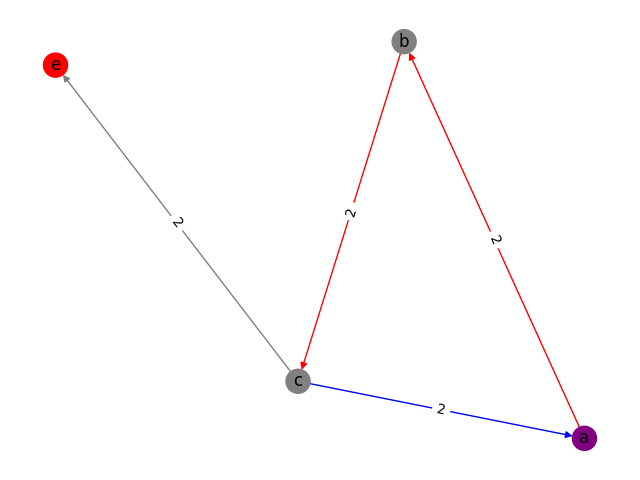
\includegraphics[width = 0.5\textwidth]{\detokenize{images/Figure_1.png}}}
\end{tabular}
  
  \caption{Running main.py on input.txt file (a) result in figure (b) }
  \label{fig:d}
\end{figure}
